%%% LaTeX Template: Two column assignment for BRSU
%%% Based on two column article from: http://www.howtotex.com/
%%% Preamble
\documentclass[	DIV=calc,%
				paper=a4,%
				fontsize=11pt,%
				twocolumn]{article}	 % KOMA-article class

\usepackage{lipsum}	% Package to create dummy text
\usepackage{blindtext}
\usepackage[english]{babel}	                          % English language/hyphenation
\usepackage[protrusion=true,expansion=true]{microtype} % Better typography
\usepackage{amsmath,amsfonts,amsthm}					 % Math packages
\usepackage[pdftex]{graphicx}	                          % Enable pdflatex
\usepackage[svgnames]{xcolor}	                          % Enabling colors by their 'svgnames'
\usepackage[small,tableposition=top,labelfont=bf,up,textfont=it,up]{caption}
% Custom captions under/above floats
\usepackage{epstopdf}	 % Converts .eps to .pdf
\usepackage{subfig}	     % Subfigures
\usepackage{booktabs}	 % Nicer tables
\usepackage{fix-cm}       % Custom fontsizes
\usepackage{listings}
\usepackage{soul}
\usepackage{float}
\usepackage{subfig}
\newsavebox{\measurebox}

%%% Custom sectioning (sectsty package)
\usepackage{sectsty}	 % Custom sectioning (see below)
\allsectionsfont{%% Change font of al section commands
	\usefont{OT1}{phv}{b}{n}%% bch-b-n: CharterBT-Bold font
	}

\sectionfont{%% Change font of \section command
	\usefont{OT1}{phv}{b}{n}%% bch-b-n: CharterBT-Bold font
	}


\definecolor{brsugrey}{rgb}{0.9, 0.9, 0.9}
\definecolor{brsublue}{rgb}{0, 0.594, 0.949}


\newcommand{\upperRomannumeral}[1]{\uppercase\expandafter{\romannumeral#1}}

%%% Headers and footers
\usepackage{fancyhdr} % Needed to define custom headers/footers
	\pagestyle{fancy} % Enabling the custom headers/footers
\usepackage{lastpage}	

% Header (empty)
\lhead{}
\chead{}
\rhead{}
% Footer (you may change this to your own needs)
\lfoot{\footnotesize 
\texttt{PR} % Set to the course abbreviation 
\textbullet ~ Moriarty % Set to your name
\textbullet ~ Assignment \upperRomannumeral{4}} % Set the assignment number
\cfoot{}
\rfoot{\footnotesize page \thepage\ of \pageref{LastPage}}	% "Page 1 of 2"
\renewcommand{\headrulewidth}{0.0pt}
\renewcommand{\footrulewidth}{0.4pt}
\renewcommand{\thesubsection}{\thesection.\alph{subsection}}

%%% Creating an initial of the very first character of the content
\usepackage{lettrine}
\newcommand{\initial}[1]{%
     \lettrine[lines=3,lhang=0.3,nindent=0em]{
     				\color{brsublue}
     				{\textsf{#1}}}{}}

%%% Title, author and date metadata
\usepackage{titling}	% For custom titles

\newcommand{\HorRule}{\color{brsublue}% Creating a horizontal rule
					 \rule{\linewidth}{1pt}%
					 \color{black}
					 }

\pretitle{\vspace{-100pt} \begin{flushleft} \HorRule 
				\fontsize{25}{25} \usefont{OT1}{phv}{b}{n} \color{gray} \selectfont 
				}
\title{Probabilistic Reasoning
\\ Assignment ~\upperRomannumeral{4}}% Title of your article goes here
\posttitle{\par\end{flushleft}\vskip 0.5em}

\preauthor{\begin{flushleft}
\large \lineskip 0.25em \usefont{OT1}{phv}{b}{sl} \color{brsublue}}
\author{Alexander Moriarty }	% Author name goes here
\postauthor{\footnotesize \usefont{OT1}{phv}{m}{sl} \color{Black} 
BRS University of Applied Sciences % Institution of author
\\email: alexander@dal.ca ~github: @moriarty
\par\end{flushleft}\HorRule}

\date{\today} 
\onecolumn
%%% Begin document
\begin{document}
\maketitle
\thispagestyle{fancy} % Enabling the custom headers/footers for the first page 

%\setcounter{section}{5}

\section{Car Diagnosis}
\paragraph{Consider the network for car diagnosis shown in Figure 14.18. }
\subsection{}
\paragraph{Extend the network with the Boolean variables \emph{IcyWeather} and \emph{StarterMotor}.}
~\\
\begin{figure}[h]
  \centering
  \caption{Car Diagnosis Network Extended}
  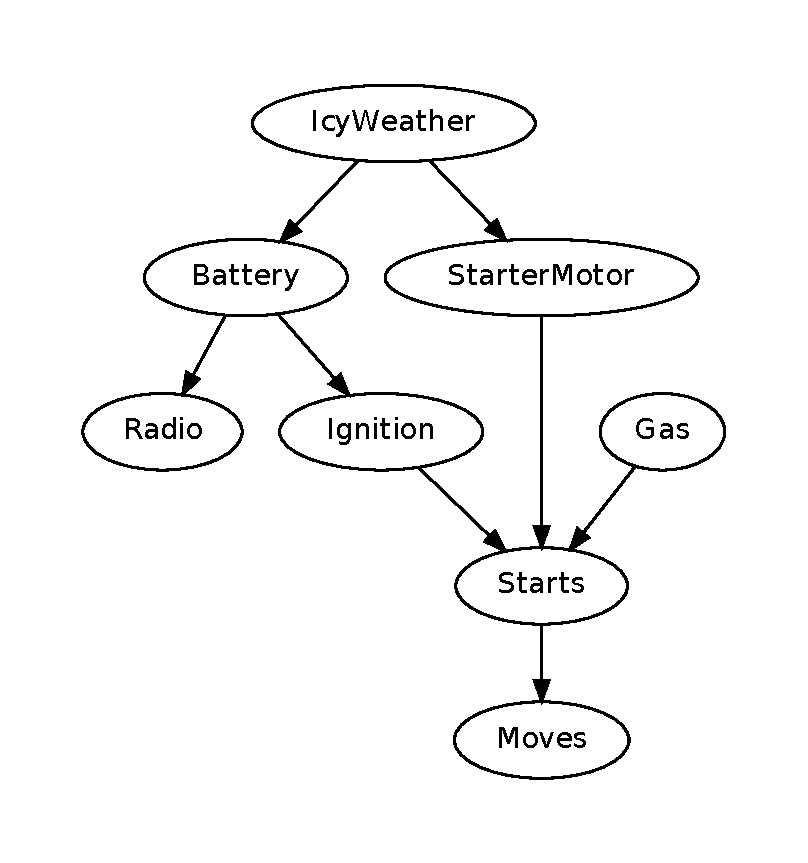
\includegraphics[width=0.5\textwidth]{./car_diagnosis}
\end{figure}
\newpage
\subsection{}
\paragraph{Give reasonable conditional probability tables for all the nodes.}
~\\
\begin{table}[H]
\centering
\subfloat[Icy Weather~(IW)]{
\begin{tabular}{|c|}
\hline
P(IcyWeather) \\ \hline
0.25 \\ \hline
\end{tabular}}
\qquad
\subfloat[Battery~(B)]{
\begin{tabular}{|c|c|}
\hline
IW		& P(Battery) \\ \hline
t 		& 0.90   \\ 
f 		& 0.99   \\ \hline
\end{tabular}}
\qquad
\subfloat[Starter Motor~(SM)]{
\begin{tabular}{|c|c|}
\hline
IW		& P(StarterMotor) \\ \hline
t 		& 0.90   \\ 
f 		& 0.99   \\ \hline
\end{tabular}}
\qquad
\subfloat[Radio~(R)]{
\begin{tabular}{|c|c|}
\hline
B	& P(Radio) \\ \hline
t 		& 0.99   \\ 
f 		& 0.01   \\ \hline
\end{tabular}}
\quad
\subfloat[Ignition~(I)]{
\begin{tabular}{|c|c|}
\hline
B	& P(Ignition) \\ \hline
t 		& 0.99   \\ 
f 		& 0.01   \\ \hline
\end{tabular}}
\quad
\subfloat[Gas~(G)]{
\begin{tabular}{|c|}
\hline
P(Gas) \\ \hline
0.95 \\ \hline
\end{tabular}}
\quad
\subfloat[Starts~(S)]{
\begin{tabular}{|ccc|c|}
\hline
I & SM & G & P(Starts) \\ \hline
t & t  & t & 0.99 \\ 
t & t  & f & 0.00 \\ 
t & f  & t & 0.00 \\ 
t & f  & f & 0.00 \\ 
f & t  & t & 0.00 \\ 
f & t  & f & 0.00 \\ 
f & f  & t & 0.00 \\ 
f & f  & f & 0.00 \\\hline
\end{tabular}}
\quad
\subfloat[Moves~(M)]{
\begin{tabular}{|c|c|}
\hline
S & P(Moves) \\ \hline
t & 0.99 \\
f & 0.01 \\ \hline
\end{tabular}}
\caption{Conditional probability tables for car diagnosis network}
\label{table:first}
\end{table}

\subsection{}
\paragraph{Many independent values are contained in the joint probability distribution for eight Boolean nodes, assuming that no conditional independence relations are known to hold among them?}
~\\
There are $2^{8}$ possible values for the 8 boolean variables, but we know they will all sum up to 1 so we get one value for free.
\begin{eqnarray}
2^{8}-1 &=& 255
\end{eqnarray}
\newpage
\subsection{}
\paragraph{How many independent probability values do your network tables contain?}
~\\
\begin{table}[H]
\centering
\begin{tabular}{|c|c|c|}
\hline
From Table: \ref{table:first} &  & Values \\ \hline
a & $2^{0}$ & 1 \\
b & $2^{1}$ & 2 \\
c & $2^{1}$ & 2 \\
d & $2^{1}$ & 2 \\
e & $2^{1}$ & 2 \\
f & $2^{0}$ & 1 \\ 
g & $2^{3}$ & 8 \\
h & $2^{1}$ & 2 \\ \hline
Total & $2\cdot2^{0}+5\cdot2^{1}+2^{3}$ & 20 \\ \hline
\end{tabular}
\caption{Number of independent probability values}
\label{table:second}
\end{table}

\subsection{}
\paragraph{The conditional distribution for \emph{Starts} could be described as a \emph{noisy-AND} distribution. Define this family in general and relate it to the \emph{noisy-OR} distribution.}
~\\
Because all of the variables must be true for the motor to start we can think of it as:
\setcounter{equation}{0}
\begin{eqnarray}
Starts &\approx & Ignition \wedge StarterMotor \wedge Gas
\end{eqnarray}
Using De Morgan's we know this could equivalently use OR:
\begin{eqnarray}
Starts &\approx & \neg ( \neg Ignition \vee \neg StarterMotor \vee \neg Gas ) 
\end{eqnarray}
It's noisy because there is still the possibility that all variables are true/false and the motor doesn't start. 

\newpage
\section{Nuclear Power Station}
\paragraph{In your local nuclear power station, there is an alarm that senses when a temperature gauge exceeds a given threshold.
The gauge measures the temperature of the core. Consider the Boolean variables $A(alarm~sounds)$, $FA(alarm~is~faulty)$, and $FG(gauge~is~faulty)$ and the multi-valued nodes $G(gauge~reading)$ and $T(actual~core~temperature)$
}
~\\
\begin{figure}[h]
  \centering
  \caption{.}
  \sbox{\measurebox}{
  \begin{minipage}[b]{0.4\textwidth}
  \subfloat[Bayesian Network of Power Domain]{
  	\label{fig:q2_a}
  	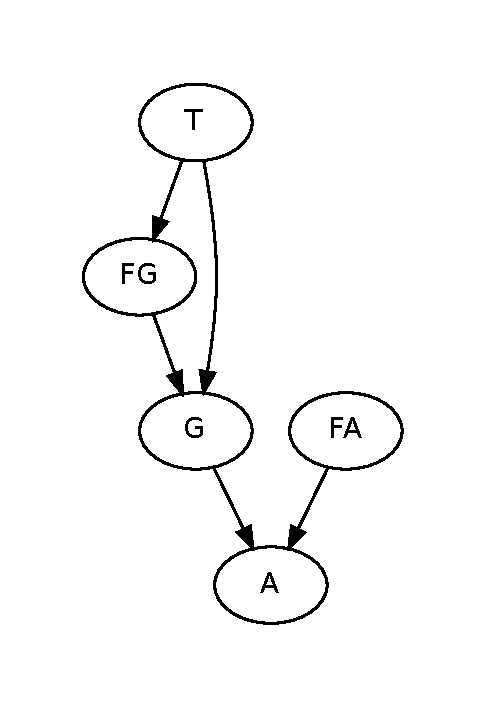
\includegraphics[width=0.7\textwidth]{./nuclear_power}
  }
  \end{minipage}}
  \usebox{\measurebox}\qquad
  \begin{minipage}[b][\ht\measurebox][s]{0.4\textwidth}
  \subfloat[Question 2.c]{
  \label{table:q2_c}
\begin{tabular}{*5c}
{} & \multicolumn{2}{c}{$T=Normal$} & \multicolumn{2}{c}{$T=High$} \\
{} & $FG$ & $\neg FG$ & $FG$ & $\neg FG$ \\
\midrule
$G=Normal$ & $1-y$ & $1-x$ & $y$ & $x$ \\
$G=High$ & $y$ & $x$ & $1-y$ & $1-x$ \\
\bottomrule
\end{tabular}}

\vfill

  \subfloat[Question 2.d]{
  \label{table:q2_d}
\begin{tabular}{*5c}
{} & \multicolumn{2}{c}{$T=Normal$} & \multicolumn{2}{c}{$T=High$} \\
{} & $FG$ & $\neg FG$ & $FG$ & $\neg FG$ \\
\midrule
$A$ & 0 & 0 & 0 & 1 \\
$\neg A$ & 1 & 1 & 1 & 0 \\
\bottomrule
\end{tabular}}
  \end{minipage}  

\end{figure}


\subsection{}
\paragraph{Draw a Bayesian network for this domain, given that the gauge is more likely to fail when the core tempurature gets too high.}
~\\
Please see Figure \ref{fig:q2_a}
\subsection{}
\paragraph{Is your network a polytree?}
~\\
No, there are two paths from $T$ to $G$. 
\subsection{}
\paragraph{Suppose there are just two possible actual and measured temperatures, normal and high; the probability that the gauge gives the correct temperature is $x$ when it is working, but $y$ when it is faulty. Give the conditional probability table associated with $G$}
~\\
% Answer
Please see Figure \ref{table:q2_c}
\subsection{}
\paragraph{Suppose the alarm works correctly unless it is faulty, in which case it never
sounds. Give the conditional probability table associated with $A$.}
~\\
% Answer
Please see Figure \ref{table:q2_d}
\subsection{}
\paragraph{Suppose the alarm and gauge are working and the alarm sounds. Calculate
an expression for the probability that the temperature of the core is too high, in
terms of the various conditional probabilities in the network.}
~\\
% Answer
We know $FA$ and $A$ do not influence $T$:
\setcounter{equation}{0}
\begin{eqnarray}
P( T \mid A, \neg {FA}, \neg {FG} ) &=& P( T \mid G, \neg {FG})\\
P( T \mid G, \neg {FG}) &=& P(G \mid T, \neg{FG})P(T\mid\neg{FG})\\
P( T \mid G, \neg {FG}) &=& P(G \mid T, \neg{FG})P(\neg{FG}\mid{T})P(T)\\
P( T \mid G, \neg {FG}) &=& \frac{P(G \mid T, \neg{FG})P(\neg{FG}\mid{T})P(T)}
{P(G \mid T, \neg{FG})P(\neg{FG}\mid{T})P(T) + P(G \mid\neg{T}, \neg{FG})P(\neg{FG}\mid\neg{T})P(\neg{T})}
\end{eqnarray}


\end{document}
